\documentclass[12pt]{article}
\usepackage{amsmath}
\usepackage{geometry}
\usepackage{graphicx}
\usepackage{hyperref}
\usepackage[latin1]{inputenc}
\usepackage{listings}
\usepackage[dvipsnames]{xcolor}
\renewcommand{\labelitemi}{$\textendash$}
\geometry{
    a4paper,
    total={170mm,257mm},
    left=20mm,
    right=20mm,
    top=5mm,
    bottom=15mm
}

\title{CS7DS2: Week 2 Assignment}
\author{Conor McCauley - 17323203}
\date{February 6, 2022}

\begin{document}

\maketitle

\section*{Question (a)}

\noindent (i) Using \textit{SymPy} we can initialise a symbol, $x$, and define a function of that symbol, $y = x^4$. We can then use the \texttt{diff()} function to find the derivative of $y(x)$:

\lstset{basicstyle=\footnotesize,xleftmargin=.35in}
\begin{lstlisting}[language=Python]
import sympy as sp
x = sp.symbols('x')
y = x**4
dydx = sp.diff(y, x)
print(dydx)
\end{lstlisting}

The above code outputs the result $4x^3$.

\noindent (ii) Using a value range of $-2 \leq x \leq 2$ we can use the \texttt{sympy.plotting} module to plot the calculated derivative from (i). We can also estimate the derivative using finite difference with $\delta=0.01$ and the equation $(y(x + \delta) - y(x)) / \delta$ which is done using the following code:

\lstset{basicstyle=\footnotesize,xleftmargin=.35in}
\begin{lstlisting}[language=Python]
delta = 0.01
dydx_estimate = ((x + delta)**4 - x**4) / delta
\end{lstlisting}

The \texttt{compare\_plots()} function in \texttt{a.py} produced the following plot when $\delta=0.01$:

\begin{center}
    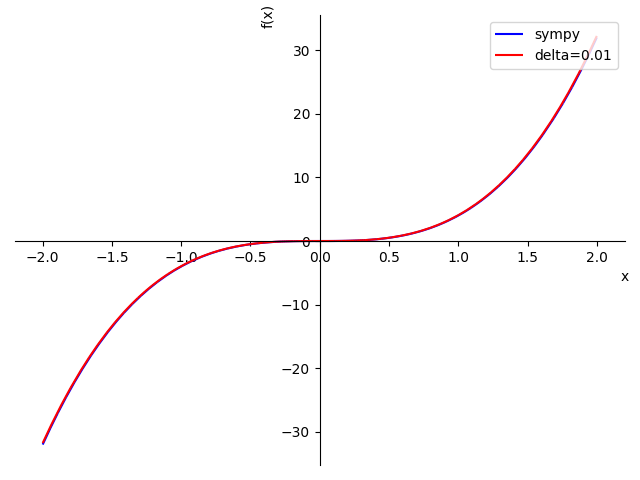
\includegraphics[scale=0.55]{figs/a/a_ii.png}
\end{center}

From the above plot it is evident that, at least within the range $-2 \leq x \leq 2$, the estimated derivative is almost identical to the calculated derivative.

\noindent (iii) As in (ii), we can use the \texttt{compare\_plots()} function to plot the estimated derivatives for $\delta \in \{0.001, 0.01, 0.1, 1\}$ and $-2 \leq x \leq 2$. The following plot is produced:

\begin{center}
    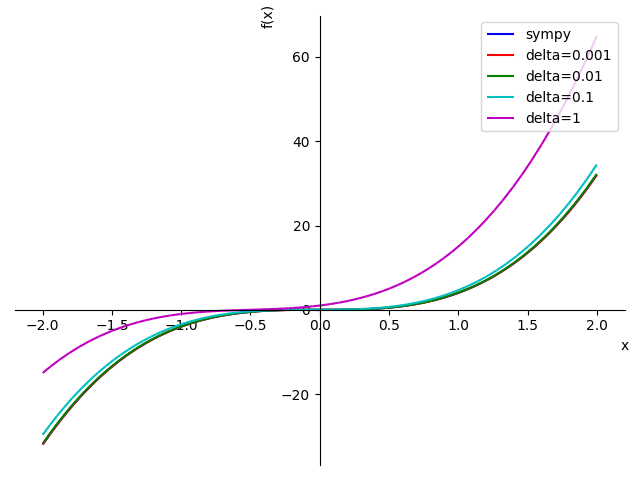
\includegraphics[scale=0.55]{figs/a/a_iii.png}
\end{center}

When $\delta \leq 0.01$ the results are almost identical to the calculated derivative however we can see that the estimated values begin to diverge from the actual values when $\delta=0.1$ and when $\delta=1$ the estimated values are very inaccurate. Increasing $\delta$ reduces the accuracy of the estimated values due to an increase in the actual difference between the values of $y(x + \delta)$ and $y(x)$.

\section*{Question (b)}

\noindent (i) The \texttt{gradient\_descent()} function takes a function $y(x)$ and its derivative $\frac{dy}{dx}$ as parameters along with the initial value of $x$, the step size $\alpha$ and the number of gradient descent iterations to run. During each iteration the value of $x$ is decremented by the product of $\alpha$ and the value of the derivative of $x$. The values of $x$ and $y(x)$ during each iteration are added to arrays and then returned at the end of the function where they can be plotted.

\lstset{basicstyle=\footnotesize,xleftmargin=.35in}
\begin{lstlisting}[language=Python]
def gradient_descent(y, dy, x, alpha, num_iters):
    xs, ys = [x], [y(x)]
    for _ in range(num_iters):
        step = alpha * dy(x)
        x -= step
        xs.append(x)
        ys.append(y(x))
    return xs, ys
\end{lstlisting}

\noindent (ii) With $x_0=1$ and $\alpha=0.1$ the gradient descent algorithm is run for 100 iterations. Lambda functions for 
$y=x^4$ and $\frac{dy}{dx}=4x^3$ are also passed as parameters. The value of $y(x)$ decreases and quickly approaches its minimum in less than 10 iterations. The value of $x$ decreases more slowly due to the fact that, as $x$ decreases, the amount that is decremented from $x$ at each iteration, $\alpha\cdot4x^3$, decreases at a much faster rate.

\begin{center}
    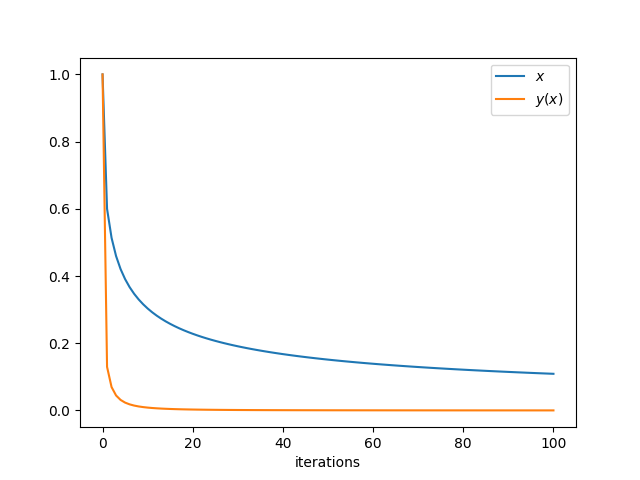
\includegraphics[scale=0.55]{figs/b/b_ii.png}
\end{center}

\noindent (iii) The gradient descent algorithm was run for 100 iterations for values of $\alpha \in \{0.001, 0.01, 0.1\}$ and values of $x_0 \in \{0.1, 0.5, 1\}$. A separate plot was created for each value of $\alpha$ and the different values of $x$ and $y(x)$ at each iteration were displayed.

When $\alpha = 0.001$ the change in $x$ after each iteration is very small resulting in neither the $x_0=1$ or $x_0=0.5$ experiments converging after 100 iterations. It's worth noting, however, that even when $x_0=0.1$ all values of $y(x)$ are so small that they're indistinguishable from 0 on the plot below.

\begin{center}
    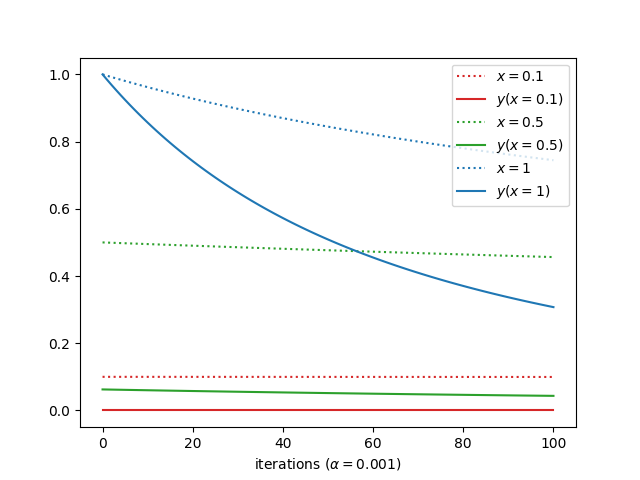
\includegraphics[scale=0.55]{figs/b/b_iii_1.png}
\end{center}

When $\alpha = 0.01$ the change in $x$ after each iteration is relatively small and, as such, both the $x_0=0.5$ and $x_0=1$ experiments take over 80 trials to appear to converge on the minimum with the $x_0=1$ experiment barely converging within 100 trials. Again, when $x_0=0.1$, the plotted values of $y(x)$ are indistinguishable from 0.

\begin{center}
    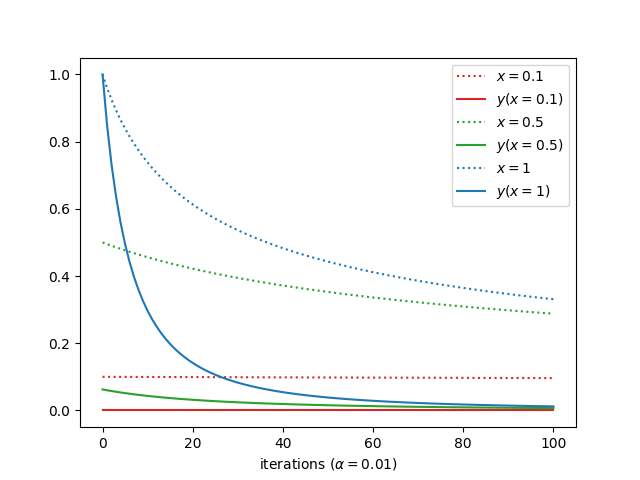
\includegraphics[scale=0.55]{figs/b/b_iii_2.png}
\end{center}

When $\alpha = 0.1$, like in part (ii), all of the experiments rapidly converge on the minimum regardless of the value of $x_0$.

\begin{center}
    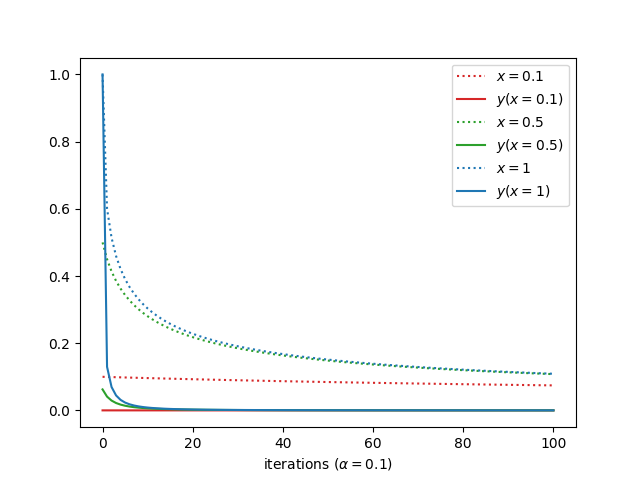
\includegraphics[scale=0.55]{figs/b/b_iii_3.png}
\end{center}

If $\alpha$ is too small, as in the first two plots, then $x$ is decremented too slowly during each iteration resulting in much slower, if any, convergence. Out of the above examples it appears that the optimal value of $\alpha$ is 0.1. The initial value of $x$ does not appear to have too much of an effect on the rate of convergence since, at least in the example, the larger the value of $x$ is the larger its derivative will be at each iteration.

\section*{Question (c)}

\noindent (i) The gradient descent algorithm was run for 100 iterations for $\alpha=0.1$, $x_0=1$ and values of $\gamma \in \{0.5, 1, 3\}$. From the below plot it appears that the larger $\gamma$ is the quicker it converges on the minimum. The derivative of $y(x)$, $2\gamma x$, will be larger when $\gamma$ is larger and, given that $x_0=1$ for each experiment, the value of $x$ will be decremented by more during each iteration due to $\gamma$ being larger, leading to quicker convergence.


\begin{center}
    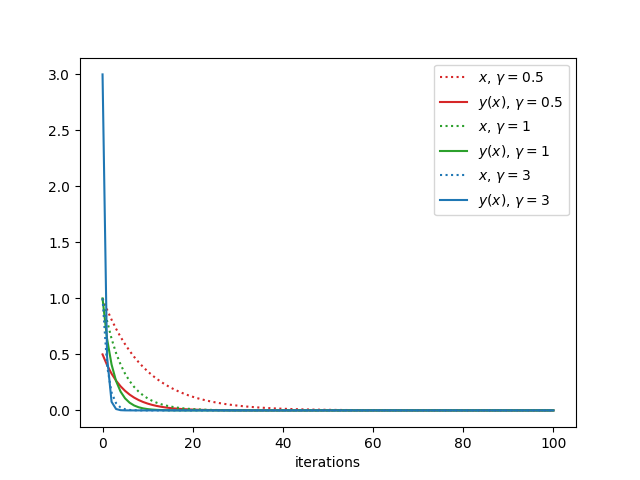
\includegraphics[scale=0.55]{figs/c/c_i.png}
\end{center}

\noindent (ii) As in (i), $\alpha=0.1$ and $x_0=1$. The derivative of $\gamma|x|$ is $\frac{\gamma x}{|x|}$. From the below plot it can be seen that for larger values of $\gamma$ the value of $y(x)$ initially decreases faster due to $\frac{x}{|x|}$ being constant when $x > 0$. However, at a certain point the value of $x$ begins to oscillate back and forth around the minimum, 0, indefinitely without every reaching it. This in turn prevents the value of $y(x)$ from converging on the minimum.

\begin{center}
    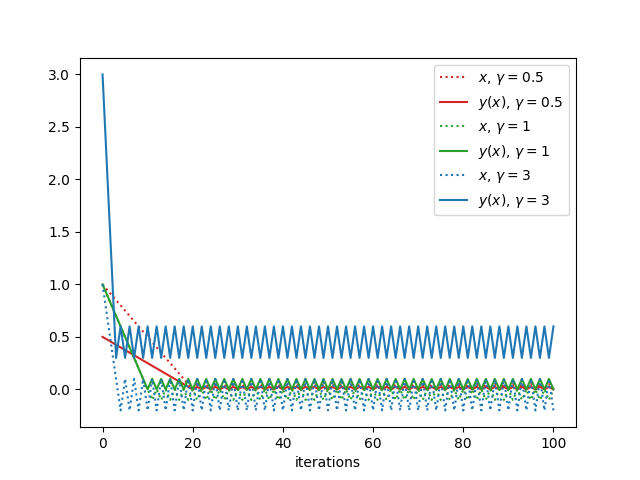
\includegraphics[scale=0.55]{figs/c/c_ii.png}
\end{center}

\section*{Appendix A: Code}

\subsection*{Code for (a)}

\lstset{basicstyle=\footnotesize,xleftmargin=0in}
\begin{lstlisting}[language=Python]
import sympy as sp
import sympy.plotting as plt

# (i)
x = sp.symbols('x')
y = x**4
dydx = sp.diff(y, x)
print(dydx)

# (ii) and (iii)
def compare_plots(x, dydx, deltas):
    colors = ['b', 'r', 'g', 'c', 'm']
    plot_range = (x, -2, 2)
    plots = plt.plot(dydx, plot_range, show=False,
                    label='sympy', line_color=colors[0])
    for delta, color in zip(deltas, colors[1:]):
        dydx_estimate = ((x + delta)**4 - x**4) / delta
        plot = plt.plot(dydx_estimate, plot_range, show=False,
                        label=f'delta={delta}', line_color=color)
        plots.append(plot[0])
    plots.legend = True
    plots.show()

# (ii)
compare_plots(x, dydx, [0.01])

# (iii)
compare_plots(x, dydx, [0.001, 0.01, 0.1, 1])
\end{lstlisting}

\subsection*{Code for (b) and (c)}

\lstset{basicstyle=\footnotesize}
\begin{lstlisting}[language=Python]
import matplotlib.pyplot as plt

def gradient_descent(y, dy, x, alpha, num_iters):
    xs, ys = [x], [y(x)]
    for _ in range(num_iters):
        step = alpha * dy(x)
        x -= step
        xs.append(x)
        ys.append(y(x))
    return xs, ys

def b_ii():
    N = 100
    iters = list(range(N + 1))
    y = lambda x: x**4
    dy = lambda x: 4*(x**3)
    xs, ys = gradient_descent(y, dy, x=1, alpha=0.1, num_iters=N)
    plt.plot(iters, xs)
    plt.plot(iters, ys)
    plt.legend(['$x$', '$y(x)$'])
    plt.xlabel('iterations')
    plt.show()
    
def b_iii():
    N = 100
    iters = list(range(N + 1))
    y = lambda x: x**4
    dy = lambda x: 4*(x**3)
    for alpha in [0.001, 0.01, 0.1, 0.5]:
        for x, color in zip([0.1, 0.5, 1], ['tab:red', 'tab:green', 'tab:blue']):
            xs, ys = gradient_descent(y, dy, x=x, alpha=alpha, num_iters=N)
            plt.plot(iters, xs, linestyle='dotted', color=color)
            plt.plot(iters, ys, color=color)
        plt.legend([
            '$x=0.1$', '$y(x=0.1)$',
            '$x=0.5$', '$y(x=0.5)$',
            '$x=1$', '$y(x=1)$',
        ])
        plt.xlabel(f'iterations ($\\alpha={alpha}$)')
        plt.show()

def c(is_part_i):
    N = 100
    iters = list(range(N + 1))
    gammas = [0.5, 1, 3]
    colors = ['tab:red', 'tab:green', 'tab:blue']
    for gamma, color in zip(gammas, colors):
        if is_part_i:
            y = lambda x: gamma*(x**2)
            dy = lambda x: 2*gamma*x
        else:
            y = lambda x: gamma*abs(x)
            dy = lambda x: (gamma*x)/abs(x)
        xs, ys = gradient_descent(y, dy, x=1, alpha=0.1, num_iters=N)
        plt.plot(iters, xs, linestyle='dotted', color=color)
        plt.plot(iters, ys, color=color)
    plt.legend([
        '$x,\\, \\gamma=0.5$', '$y(x),\\, \\gamma=0.5$',
        '$x,\\, \\gamma=1$', '$y(x),\\, \\gamma=1$',
        '$x,\\, \\gamma=3$', '$y(x),\\, \\gamma=3$'
    ])
    plt.xlabel('iterations')
    plt.show()

b_ii()
b_iii()
c(is_part_i=True)
c(is_part_i=False)
\end{lstlisting}

\end{document}
